\documentclass[tikz,border=12pt]{standalone}
\usepackage[T1]{fontenc}
\usepackage{mathpazo}
\usepackage{amsmath,amssymb}
\usetikzlibrary{arrows.meta, positioning, calc}

\definecolor{stblue}{HTML}{7B97AD}
\definecolor{rwgold}{HTML}{B8995E}
\definecolor{sage}{HTML}{7A9A7E}
\definecolor{dkbrown}{HTML}{3D3530}
\definecolor{wmgray}{HTML}{7B7067}
\definecolor{cream}{HTML}{F9F6F0}
\definecolor{border}{HTML}{D4C9B8}
\definecolor{terracotta}{HTML}{C47A6A}

\begin{document}
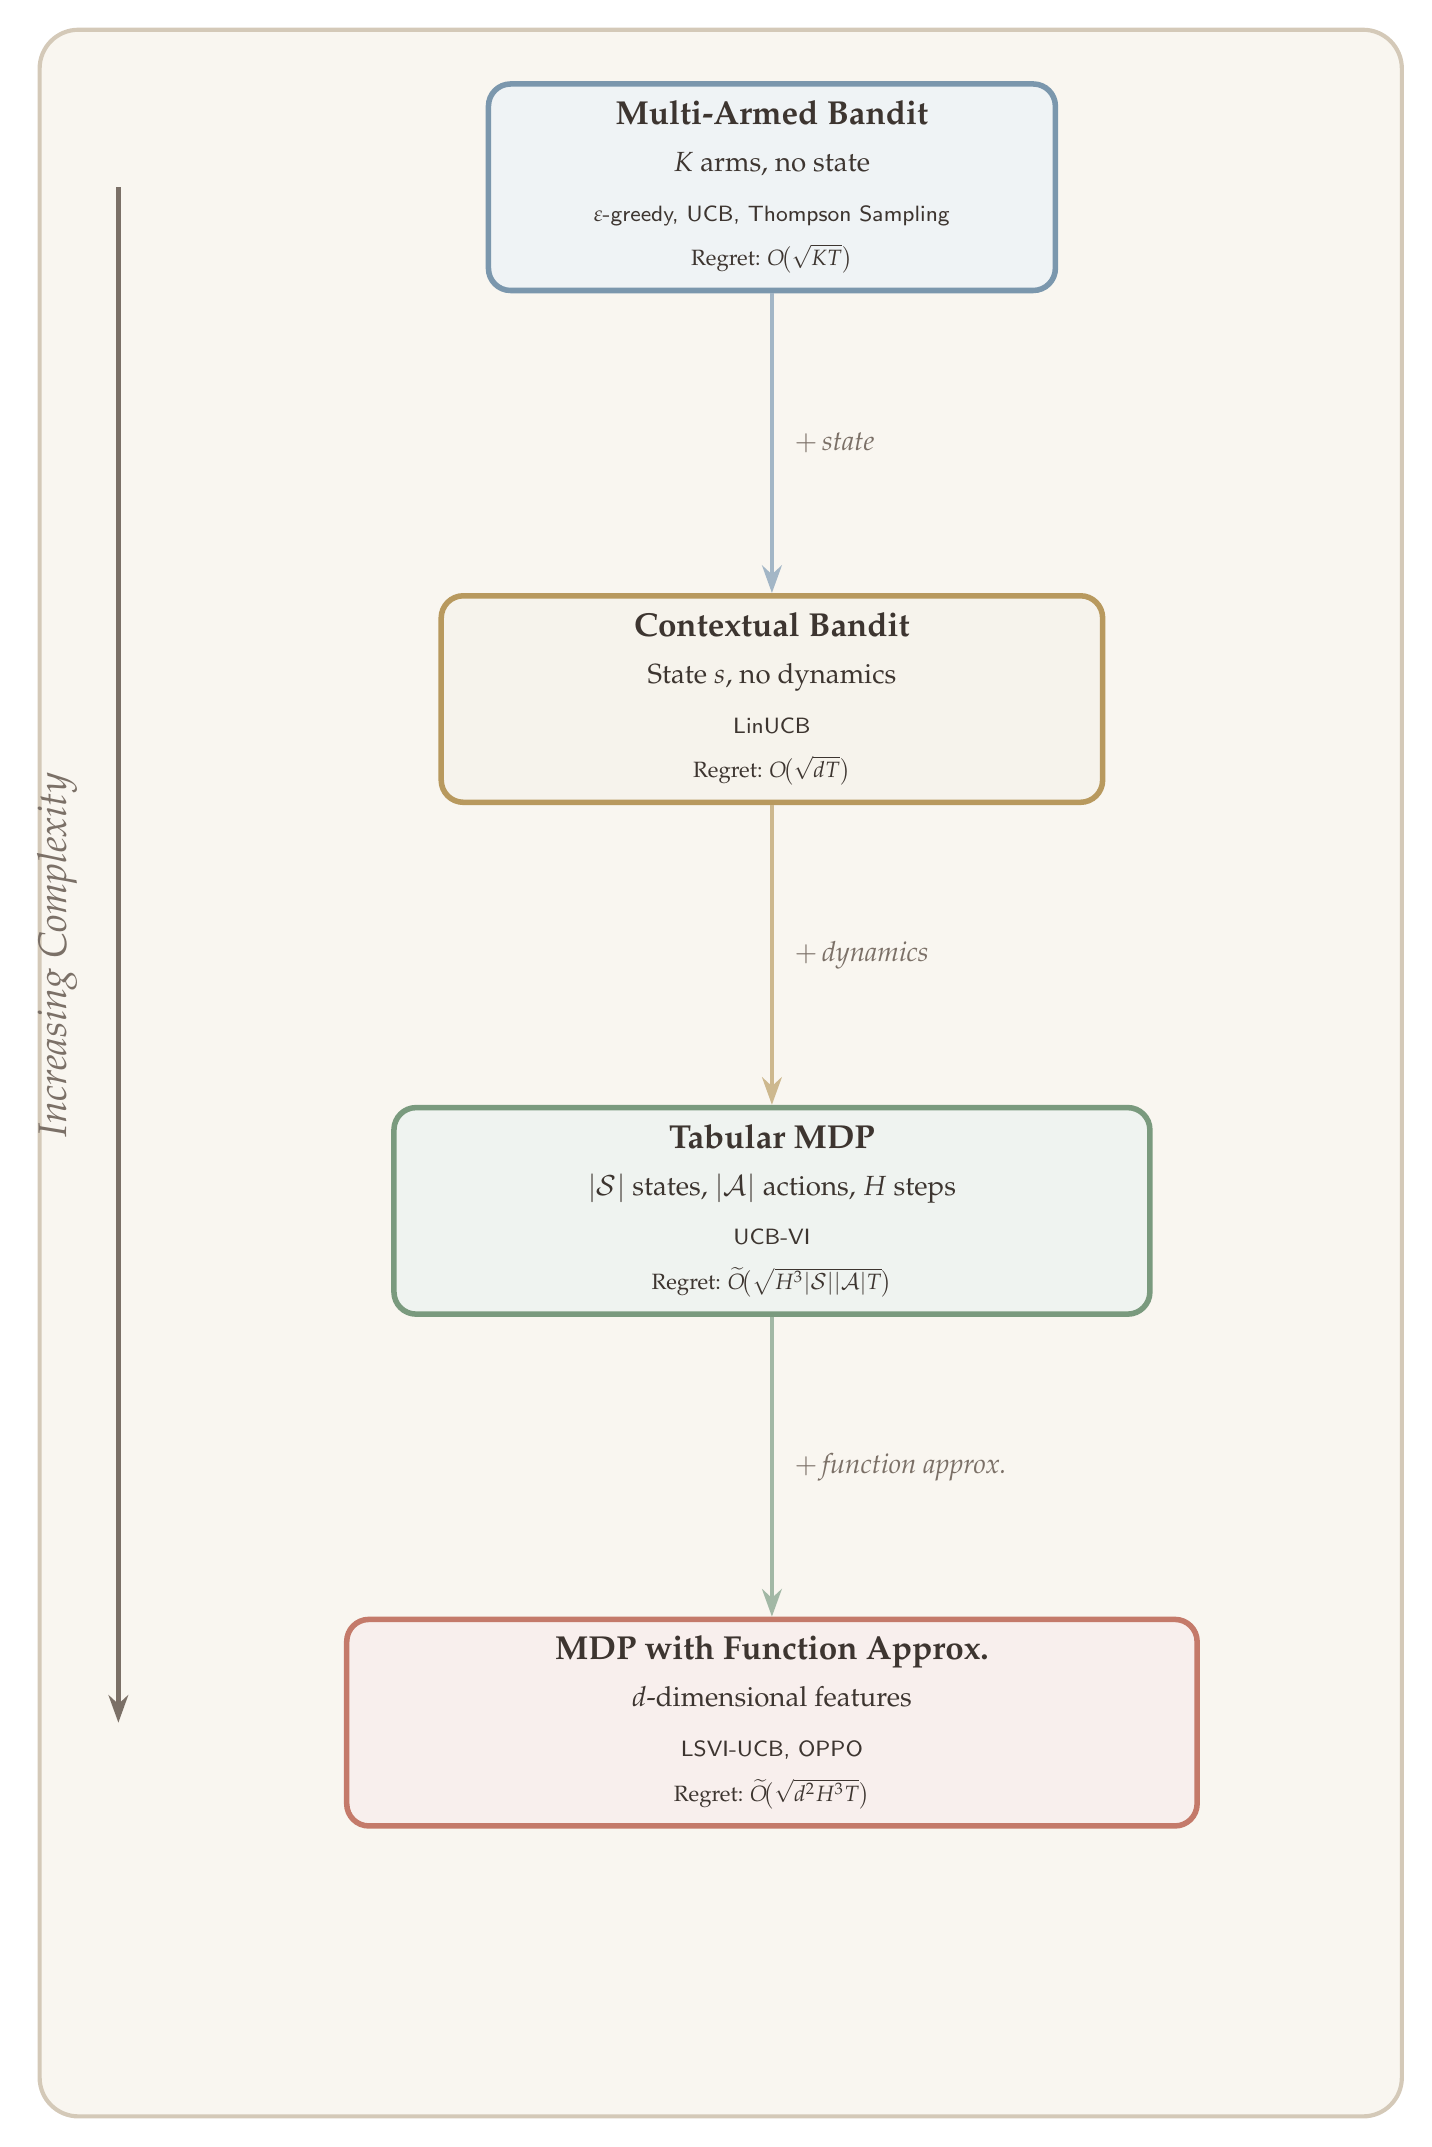
\begin{tikzpicture}[
  >={Stealth[length=3.5mm, width=2.5mm]},
  arr/.style={->, line width=1.6pt, dkbrown},
]

% =============================================
% Box styles — widths increase toward the bottom
% =============================================
\tikzset{
  levelbox/.style 2 args={
    draw=#1, line width=2pt, fill=#1!12, rounded corners=8pt,
    minimum height=24mm, font=\large, text=dkbrown,
    align=center, inner sep=6pt,
    minimum width=#2,
  },
}

% =============================================
% Background
% =============================================
\fill[cream, rounded corners=14pt] (-5.8,-23.5) rectangle (11.5,3.0);
\draw[border, rounded corners=14pt, line width=1.5pt] (-5.8,-23.5) rectangle (11.5,3.0);

% =============================================
% Level 1 (top): Multi-Armed Bandit
% =============================================
\node[levelbox={stblue}{72mm}] (mab) at (3.5,1.0)
  {\textbf{Multi-Armed Bandit}\\[3pt]
   \normalsize $K$ arms, no state\\[4pt]
   \footnotesize\textsf{$\varepsilon$-greedy, UCB, Thompson Sampling}\\[2pt]
   \footnotesize Regret: $O\!\bigl(\sqrt{KT}\bigr)$};

% =============================================
% Level 2: Contextual Bandit
% =============================================
\node[levelbox={rwgold}{84mm}] (cb) at (3.5,-5.5)
  {\textbf{Contextual Bandit}\\[3pt]
   \normalsize State $s$, no dynamics\\[4pt]
   \footnotesize\textsf{LinUCB}\\[2pt]
   \footnotesize Regret: $O\!\bigl(\sqrt{dT}\bigr)$};

% =============================================
% Level 3: Tabular MDP
% =============================================
\node[levelbox={sage}{96mm}] (tab) at (3.5,-12.0)
  {\textbf{Tabular MDP}\\[3pt]
   \normalsize $|\mathcal{S}|$ states, $|\mathcal{A}|$ actions, $H$ steps\\[4pt]
   \footnotesize\textsf{UCB-VI}\\[2pt]
   \footnotesize Regret: $\widetilde{O}\!\bigl(\sqrt{H^{3}|\mathcal{S}||\mathcal{A}|T}\bigr)$};

% =============================================
% Level 4 (bottom): MDP with Function Approx.
% =============================================
\node[levelbox={terracotta}{108mm}] (fa) at (3.5,-18.5)
  {\textbf{MDP with Function Approx.}\\[3pt]
   \normalsize $d$-dimensional features\\[4pt]
   \footnotesize\textsf{LSVI-UCB, OPPO}\\[2pt]
   \footnotesize Regret: $\widetilde{O}\!\bigl(\sqrt{d^{2} H^{3} T}\bigr)$};

% =============================================
% Arrows between levels with transition labels
% =============================================
\draw[arr, stblue!70] (mab.south) -- (cb.north)
  node[midway, right=4pt, font=\normalsize\itshape, text=wmgray] {$+\,$state};

\draw[arr, rwgold!70] (cb.south) -- (tab.north)
  node[midway, right=4pt, font=\normalsize\itshape, text=wmgray] {$+\,$dynamics};

\draw[arr, sage!70] (tab.south) -- (fa.north)
  node[midway, right=4pt, font=\normalsize\itshape, text=wmgray] {$+\,$function approx.};

% =============================================
% Left-side vertical label: "Increasing Complexity"
% =============================================
\draw[->, line width=1.6pt, wmgray] (-4.8,1.0) -- (-4.8,-18.5);
\node[font=\Large\itshape, text=wmgray, rotate=90, anchor=south] at (-5.2,-8.75)
  {Increasing Complexity};

\end{tikzpicture}
\end{document}
